
%%(GATE 2021 (ST) Q.19 ( statistics section)) \\

Simplifying $Z_n$, we have
\begin{align}
    Z_n &= -\log_e \left( \Prod_{i=1}^n (2-X_i) \right)^\frac{1}{n}\\
        &= -\frac{1}{n}\cdot \log_e \left( \Prod_{i=1}^n (2-X_i) \right)\\
        &= \sum\limits_{i=1}^n \left( (-\log_e \left( 2-X_i )\right)\cdot\frac{1}{n} \right)\\
        &= E\left(-\log_e \left( 2-X_i \right)\right)
\end{align}
Let $X$ and $Z$ be random variables. $X$ follows a uniform distribution from 0 to 2.
\begin{align}
    X &\sim \mathcal{U}[0,2],\\
    \text{and let }    Z&=-\log_e (2-X)
\end{align}
The sequence $X_n$ converges in distribution to $X$. i.e.
\begin{align}
    \lim _{n\to \infty }F_{X_n}(x)=F_X(x),
\end{align}
%The \textbf{The Law of Large Numbers} states that for large number of trials, the average obtained should be close to the expected value, and will tend to become closer to the expected value as more trials are performed.\\Therefore,
From \textbf{The Law of Large Numbers}, we have that %Keep either line 166 or 167
 for large $n$, $Z_n=E\left(-\log_e \left( 2-X_i \right)\right)$ should be close to $E\left(-\log_e \left( 2-X \right)\right)=E(Z)$. i.e.
\begin{align}
    \pr{\lim\limits_{n \to \infty}Z_n=E(Z)}=1
    \label{st2021-19:Zn_and_Z}
\end{align}

\textbf{If \pr{\lim_{n \to \infty}Y_n=Y}=1, we say that $Y_n$ almost surely converges to $Y$.} Therefore, by \eqref{st2021-19:Zn_and_Z} as $n \to \infty$, $Z_n$ almost surely converges to $E(Z)$.\\
\par The CDF of $Z$ is defined as 
\begin{align}
    F_Z(z) &= \pr{Z \leq z} \\
           &= \pr{ -\log_e(2-X)\leq z} \\
           &= \pr{\log_e(2-X) \geq -z}\\
           &= \pr{2-X \geq \exp\brak{-z}}\\
           &= \pr{X \leq 2- \exp\brak{-z}}\\
           &= F_X\brak{2- \exp\brak{-z}}
%           \\&=  1-\frac{exp(-z)}{2}
\label{st2021-19:CDF_Z}
\end{align}
The CDF for X ($F_X(x)$), a uniform distribution on $(0,2)$ is given by
\begin{align}
F_X(x) = 
\begin{cases}
0 &  x < 0 \\
\frac{x}{2} & 0 \leq x \leq 2 \\
1 & x > 2
\end{cases}
\end{align}
%
Substituting the above in \eqref{st2021-19:CDF_Z},
%
\begin{multline}
F_X\brak{2- \exp(-z)} =
\\
\begin{cases}
0 &  2- \exp(-z) < 0 \\
1- \frac{\exp(-z)}{2} & 0 \leq 2- \exp(-z) \leq 2 \\
1 & 2- \exp(-z) > 2
\end{cases}
\end{multline}
After some algebra, the above conditions yield
\begin{align}
F_Z(z) &= 
\begin{cases}
0 & z < -\log_e (2) \\
1- \frac{\exp(-z)}{2} & z \geq -\log_e (2)
\end{cases}
\label{st2021-19:CDF_Z_Final}\\
\implies f_Z(z)&=\dfrac{\text{d}(F_Z(z))}{\text{d}z}   
=\begin{cases}
0 & z < -\log_e (2) \\
\frac{\exp(-z)}{2} & z \geq -\log_e (2)
\end{cases}
\label{st2021-19:PDF_Z_Final}
\end{align}
\begin{figure}[H]
    \centering
      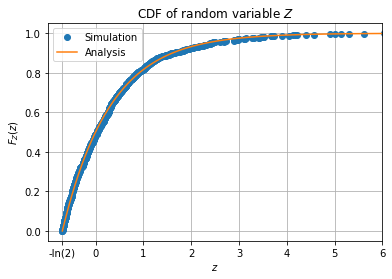
\includegraphics[width=\columnwidth]{solutions/st/2021/19/Figures/CDF_Z.png}
     \caption{$F_Z(z)$}
\end{figure}
Now calculating the expectation value for $Z$, we have
\begin{align}
    E(Z)&=\int\limits_{-\ln{2}}^{\infty}z\,f_Z(z)\,dz\\
    &=\int\limits_{-\ln{2}}^{\infty}\dfrac{z\,e^{-z}}{2}\,dz\\
    &=\left[ \dfrac{-(z+1)\,e^{-z}}{2} \right]_{-\ln{2}}^\infty\\
    &=1-\ln{(2)}\\
    &\approx0.3068
\end{align}
\par From \eqref{st2021-19:Zn_and_Z}, we have as $n \to \infty$, $Z_n$  almost surely converges to $ E(Z)=0.3068\approx0.31$(Rounded to 2 decimal places).\\
\textbf{Ans: 0.31}

